\documentclass[b5paper,xelatex,ja=standard,10pt]{bxjsarticle}
\usepackage{mystyle}  % export TEXINPUTS="./;../sty/;"
\graphicspath{{../images/}}

\usepackage{listings}
\lstset{  % グローバル設定
  columns=fixed,  % 等幅
  basewidth=0.5em,  % 字間詰め
  lineskip=-3pt,  % 行間詰め
  % フォント設定
  basicstyle={\ttfamily\small\color{DarkGray}},  % 全体設定
  keywordstyle=[1]{\color{RoyalBlue}},  % kewords[1]の設定 (Python だと予約語)
  keywordstyle=[2]{\color{VioletRed}},  % kewords[2]の設定 (Python だと組み込み関数)
  stringstyle={\color{FireBrick}},  % 文字列リテラルの設定
  commentstyle={\color{SeaGreen}},  % コメントの設定
}

%\makeatletter
%\renewcommand*\l@section{\@dottedtocline{0}{0.0em}{0.0em}}
%\makeatother

\usepackage{eso-pic}

\newcommand\BackgroundPic{%
\put(0,0){%
\parbox[b][\paperheight]{\paperwidth}{%
\vfill
\centering
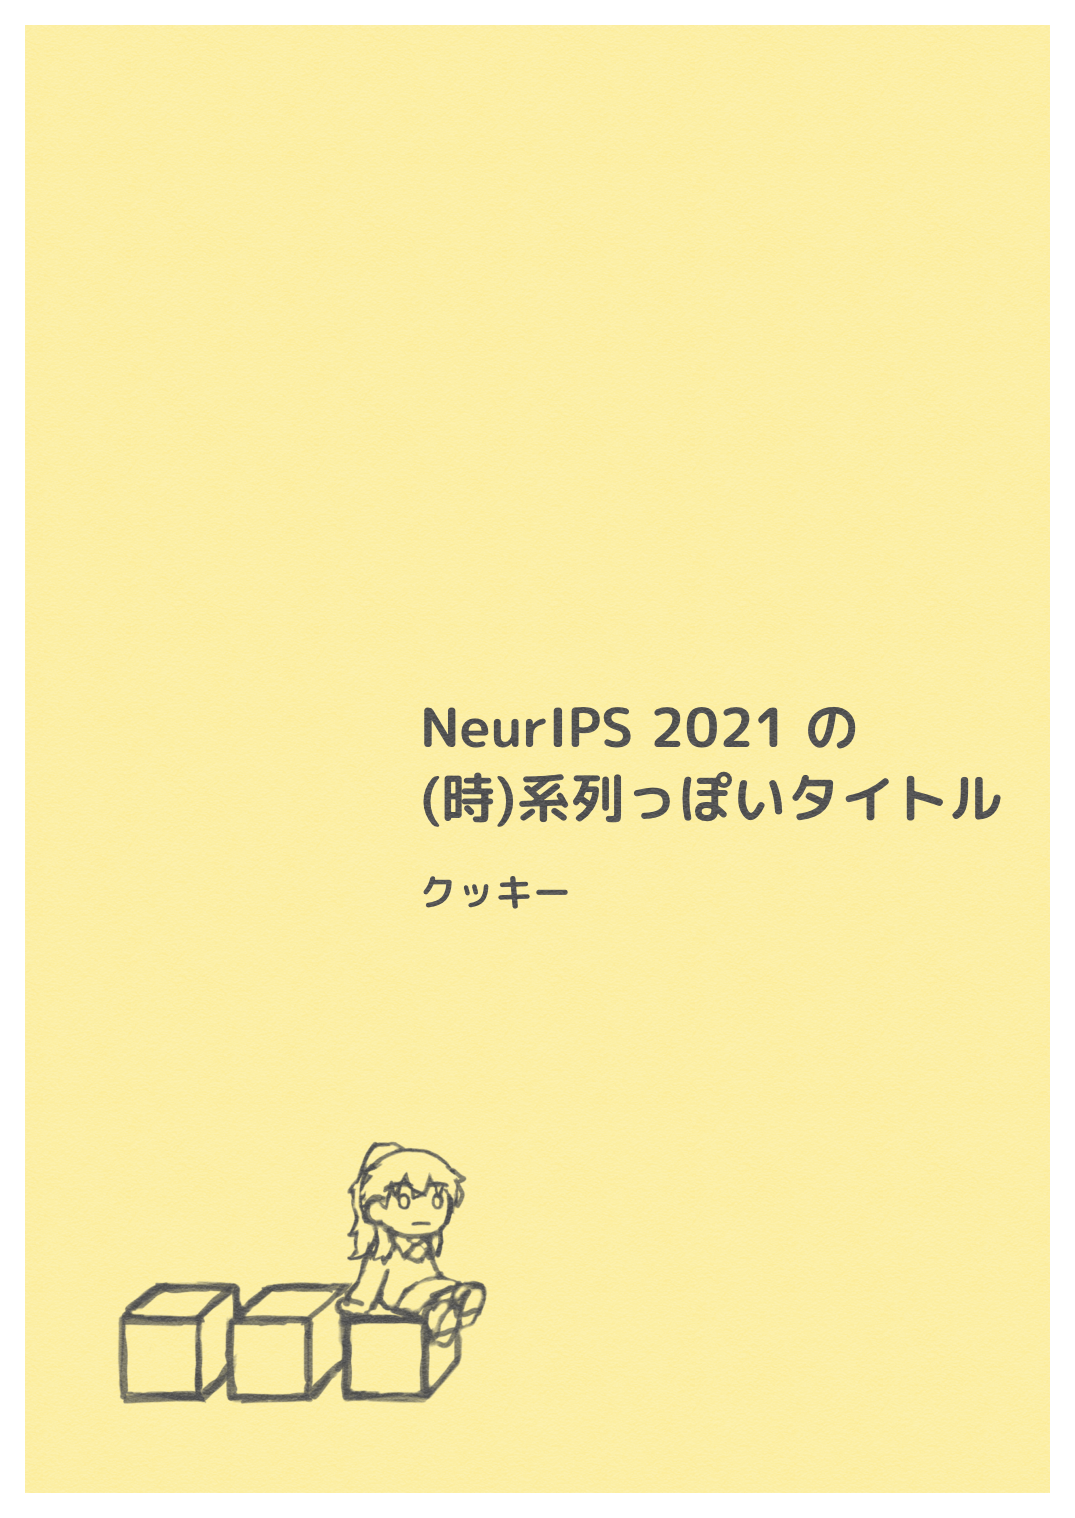
\includegraphics[width=1.0\paperwidth,height=1.0\paperheight,%
keepaspectratio]{cover.png}%
\vfill
}}}

\newcommand*{\mywatermark}{\addfontfeatures{Color=PaleVioletRed} \textbf{\small DRAFT 2022-01-21 \\ \url{https://github.com/CookieBox26/notes/tree/main/20211223_sequence_models} }}
\renewcommand*{\mywatermark}{}
\hypersetup{urlcolor=Teal}

\AddToShipoutPictureBG{
  \AtPageUpperLeft{
    \raisebox{-2.2\baselineskip}{\makebox[\paperwidth]{\begin{minipage}{14cm}\centering{\mywatermark}\end{minipage}}}
  }
}



\begin{document}


% タイトル画像
\AddToShipoutPicture*{
  \BackgroundPic
  \AtPageUpperLeft{
    \raisebox{-2.7\baselineskip}{\makebox[\paperwidth]{\begin{minipage}{14cm}\centering{\mywatermark}\end{minipage}}}
  }
  \AtPageLowerLeft{
    \raisebox{18.0\baselineskip}{\makebox[\paperwidth]{\begin{minipage}{15.4cm}\rightline{{\addCJKfontfeatures{Color=MediumVioletRed} \textbf{\huge 未完成ドラフト}}}\end{minipage}}}
  }
  \AtPageLowerLeft{
    \raisebox{14.0\baselineskip}{\makebox[\paperwidth]{
    \begin{minipage}{0.9\paperwidth}{
        \addfontfeatures{Color=MediumVioletRed}
        \addCJKfontfeatures{Color=MediumVioletRed}
        {\large
        \hspace{20em}この本は未完成ドラフトです。 \\
        \hspace{20em}目次の内容をかくことを目指しましたが \\
        \hspace{20em}第2節以降が完成していません。
        }
    }\end{minipage}
  }}
  }
}
\begin{titlepage}
\ 
\end{titlepage}


% 地の文の文字色をグレーに変更する
\addfontfeatures{Color=DarkGray}
\addCJKfontfeatures{Color=DarkGray}


% 目次
\begin{spacing}{1.0}
\tableofcontents
\end{spacing}


% まえがき
% \newpage
\vspace{6pt}
\section*{まえがき}
\addcontentsline{toc}{section}{まえがき}
\vspace{3pt}

本書は機械学習の国際会議 \, {\addfontfeatures{Color=Teal}\href{https://proceedings.neurips.cc/paper/2021}{ NeurIPS 2021}} で発表された論文から、(時)系列データを処理するためのニューラルネットワークモデル――長いのでニューラル系列モデルとよびます――に関連する研究を俯瞰しようとしたものです。が、選定した論文は網羅的でも排他的でもありません。また、論文の内容に関する記述は著者の理解であることに留意ください。著者の誤りは著者に帰属します。

本書の内容についてお気付きの点がありましたら、大変お手数ですがこの原稿があるリポジトリの Issues、または著者ブログのコメント欄までお知らせください。著者ブログへのコメントはただちには公開されません。非公開希望の方はその旨をお知らせください。非公開希望であって返信が必要な場合はご連絡先の明記をお願いいたします。

\begin{description}
    \item[ リポジトリ] \url{https://github.com/CookieBox26/notes/}
    \item[ 著者ブログ] \url{https://cookie-box.hatenablog.com/} \\ 本書に関連している記事は以下です。
    \begin{description}
        \item[  メモ前編] \url{https://cookie-box.hatenablog.com/entry/2021/11/28/191332}
        \item[  メモ後編] \url{https://cookie-box.hatenablog.com/entry/2021/12/23/124713}
    \end{description}
\end{description}

\vspace{6pt}
%\subsubsection*{登場人物紹介}
\centerline{\textbf{登場人物紹介}}

\vspace{1pt}
\begin{SERIFU}[colback=White, colbacktitle=PaleIris2, top=-1pt, bottom=0pt, left=18pt, right=10pt]{kazusa_smiley.png}
\small
この人はベイズ統計部の部長です。1年生です。とある目的のためにベイズ統計部を立ち上げ、統計や機械学習を勉強しています。ベイズ統計部には部長と副部長しかいません。姉が2人います。
\end{SERIFU}
\begin{SERIFU}[colback=White, colbacktitle=PaleGold2, top=-1pt, bottom=0pt, left=18pt, right=10pt]{takumi_smiley.png}
\small
この人はベイズ統計部の副部長です。2年生です。海外からの編入生でラクロス部に入部しようとしていましたが、部長に勧誘されてベイズ統計部に入部しました。数学が得意ですがなぜか著者を超える数学力が出せません。
\end{SERIFU}

\vspace{6pt}
\section*{第1節 \, NeurIPS 2021 のニューラル系列モデルを眺める}
\addcontentsline{toc}{section}{第1節 \, NeurIPS 2021 のニューラル系列モデルを眺める}
\vspace{5pt}

\begin{SERIFU}[colback=PaleIris, colbacktitle=PaleIris2]{kazusa_smiley.png}
(時)系列データを処理するためのニューラルネットワークモデルの動向を知るために、NeurIPS 2021 で発表された研究をみていきましょう。予稿サイトをみると、NeurIPS 2021 で発表された論文の総数は……2334本\footnote{2021年11月28日の https://proceedings.neurips.cc/paper/2021 のリンク数に基づく。}!?
\end{SERIFU}

\begin{SERIFU}[colback=PaleIris, colbacktitle=PaleIris2]{kazusa_worried.png}
あ、あまりに多いので絞り込みましょう。タイトルに time series, sequential, rnn, recurrent, transformer, attention, state space のいずれかを含む論文は……それでも 155本……。ただこの絞り込みだと画像認識, GAN, 強化学習の研究も多そうですね。それらも興味深いですが、(時)系列に関する研究を優先するべく断腸の思いでとばしていきましょう……。
\end{SERIFU}

\begin{SERIFU}[colback=PaleIris, colbacktitle=PaleIris2]{kazusa_neutral.png}
とばしても 39 本……多いですね……こう多いと何が何だかわかりません。モデルの切り口でグループ分けしてみましょう。さらにグループ内をアブストラクトからの私の理解の範囲で区分してみましょう。
\end{SERIFU}
\vspace{1pt}
\centerline{――作業後。}

\begin{SERIFU}[colback=PaleIris, colbacktitle=PaleIris2]{kazusa_smiley.png}
まず、最大勢力は Transformer ですね、検索語に含めたのでヒットするのは当然ですが、多くを占めます。特に\textbf{「セルフアテンションの計算量に対処する」}は昨年以前から引き続いて人気(?)なテーマであるようです。このサブグループは後で改めてメモしましょう。全体としては、「Transformer の性質を明らかにしようとしたもの」「訓練方法を工夫したもの」「使い方を工夫したもの」「アーキテクチャ自体を工夫したもの」「新しい用途に利用したもの」といった区分をしてみました。無論、この区分も解釈の一例であることに留意ください。
\end{SERIFU}

\addcontentsline{toc}{subsection}{グループ「Transformer」}
\vspace{1pt}
\begin{PROP}[left=0pt]{グループ「Transformer」}
\begin{itemize}
  \item Transformerの性質を理解する。
    \begin{itemize}
    \item 行列分解でパラメータを10倍削減しても性能が出ると示す \cite{AliakbarPanahi2021}。
    \item セルフアテンションを生物学的な記憶モデルと解釈する \cite{TrentonBricken2021}。
  \end{itemize}
  \vspace{6pt}
  \item Transformerの訓練方法を工夫する。
  \begin{itemize}
    \item ヘッド間で $Q, K$ の分布を一致させる正則化をする \cite{ShujianZhang2021}。
  \end{itemize}
  \vspace{6pt}
  \item Transformerの使い方を工夫する。
  \begin{itemize}
    \item グリッド分割をさらにグリッド分割する(Vision Transformer) \cite{KaiHan2021}。
    \item 機械的にプレ処理(トレンド-季節性分解)をする \cite{HaixuWu2021}。
    \item 状態空間モデルと組み合わせて時系列の長期予測等をする \cite{BinhTang2021}。
    \item データ間でセルフ(セルフ?)アテンションする \cite{JannikKossen2021}。
  \end{itemize}
  \vspace{6pt}
  \item Transformerのアーキテクチャを工夫する。
  \begin{itemize}
    \item \textbf{セルフアテンションの計算量に対処する} \cite{YifanChen2021} \cite{XuezheMa2021} \cite{SubhabrataDutta2021} \cite{SebastianJaszczur2021} \cite{BeidiChen2021} \cite{ChenZhu2021} \cite{HongyuRen2021} \, \cite{ShengjieLuo2021} \cite{TanNguyen2021}。
    \item その他Transformerのアーキテクチャを再考する。
    \begin{itemize}
      \item 言語処理に適した構造を探索する \cite{DavidSo2021}
      \item セルフアテンションの代わりにゲート付MLPにする \cite{HanxiaoLiu2021}。
      \item 時系列予測のために位相的アテンションを導入する \cite{SebastianZeng2021}。
      \item Softmax しないセルフアテンションで偏微分方程式を解く \cite{ShuhaoCao2021}。
    \end{itemize}
  \end{itemize}
  \vspace{6pt}
  \item Transformerを新しい用途に利用する。
  \begin{itemize}
    \item Transformerでガウス過程モデル適用時のカーネルを同定する \cite{FergusSimpson2021}。
  \end{itemize}
\end{itemize}
\end{PROP}
\vspace{1pt}

\begin{SERIFU}[colback=PaleIris, colbacktitle=PaleIris2]{kazusa_smiley.png}
次の勢力は RNN ですね。\textbf{「RNN を理論的に理解する」}という研究が割にみられるように感じられます。理論解析が進めばどのような系列データにどのようなニューラルアーキテクチャを用いるべきかにつながるのでしょうか……?? もちろん、「RNN を工夫する」といったより目先の実用を見据えた動機でありそうな研究もみうけられます。このグループの4研究の趣旨はそれぞれ「訓練をロバストにしたい」「表現力を上げたい」「訓練時間を短くしたい」「レジームを最大限に利用したい」といったところでしょうか。
\end{SERIFU}

\addcontentsline{toc}{subsection}{グループ「RNN」}
\vspace{1pt}
\begin{PROP}[left=0pt]{グループ「RNN」}
\begin{itemize}
  \item \textbf{RNN を理論的に理解する}。
  \begin{itemize}
    \item RNN がある再生核ヒルベルト空間におけるカーネル法であると示す \cite{AdelineFermanian2021}。
    \item スイッチング線形動的システムで RNN をリバースエンジニアリングする \cite{JimmySmith2021}。
    \item RNN が学習できると保証される関数の制約を撤廃する \cite{LifuWang2021} \cite{AbhishekPanigrahi2021}。
    \item タスクの解空間を構造化して RNN の性質を調べる \cite{EliaTurner2021}。
    \item 勾配消失/爆発しない RNN のサブセットを突き止める \cite{ZimingZhang2021}。
    \item 成長するメモリ付き固定精度 RNN がチューリング完全であると示す \cite{StephenChung2021}。
  \end{itemize}
  \vspace{6pt}
  \item RNN を工夫する。
  \begin{itemize}
    \item 訓練時に隠れ状態にノイズ添加してロバストにする \cite{SoonHoeLim2021}。
    \item RNN 自体が時間変化できるようにする \cite{AstonZhang2021}。
    \item ドロップアウトを活用してLSTMの訓練を効率化する \cite{AnupSarma2021}。
    \item 継続期間も明示的に利用するレジームスイッチングモデルを実現する \cite{AbdulFatirAnsari2021}。
  \end{itemize}
\end{itemize}
\end{PROP}
\vspace{1pt}

\begin{SERIFU}[colback=PaleIris, colbacktitle=PaleIris2]{kazusa_neutral.png}
後はその他とでもしましょうか。内容は色々なんですが……例えば Transformer と CNN の比較がありました。微分方程式で記述されるようなシステムを表現するモデルの話題も複数。それ以降は特に時系列といった研究ですね。モデルへの工夫がメインとなる研究は既に Transformer, RNN のグループに分類しましたから、ここに分類されてくるのはプレ処理/ポスト処理といった向きのもののようです。異常検知やクラスタリングについては予測といったものではないですが、たまたま目に付いて興味を引いたので選びました。
\end{SERIFU}

\addcontentsline{toc}{subsection}{その他}
\vspace{1pt}
\begin{PROP}[left=0pt]{その他}
\begin{itemize}
  \item 系列モデルを比較する。
  \begin{itemize}
    \item Transformer と CNN のロバスト性を比較する \cite{YutongBai2021}。
  \end{itemize}
  \vspace{6pt}
  \item 微分方程式で記述されるシステムをニューラルネットで実現する。
  \begin{itemize}
    \item 線形時不変連続時間システムをニューラルネットで実現する \cite{AlbertGu2021}。
    \item 連立微分方程式システムをベイズフィルタで解く \cite{JonathanSchmidt2021}。
  \end{itemize}
  \vspace{6pt}
  \item 時系列モデルの性能を向上させる汎用的なプレ処理/ポスト処理を導入する。
  \begin{itemize}
    \item 機械的に汎用的なプレ処理(成分クラスタリング)をする \cite{ZhiboZhu2021}。
    \item 誤差の自己相関を調整する \cite{FanKengSun2021}。
  \end{itemize}
  \vspace{6pt}
  \item 時系列の異常検知を工夫する。
  \begin{itemize}
    \item 時系列のオンライン異常検知の偽陽性率を制御する \cite{QuentinRebjock2021}。
  \end{itemize}
  \vspace{6pt}
  \item 時系列のクラスタリングを工夫する。
  \begin{itemize}
    \item 時系列を生成する混合分布を推定するためのコアセットを構築する \cite{LingxiaoHuang2021}。
  \end{itemize}
\end{itemize}
\end{PROP}
\vspace{1pt}

\begin{SERIFU}[colback=PaleIris, colbacktitle=PaleIris2]{kazusa_neutral.png}
最後に\textbf{「セルフアテンションの計算量に対処する」}を回収しましょう。そもそも Transformer の計算量が取り沙汰されるのは $\mathrm{Softmax} \left( Q K ^\top / \sqrt{d} \right) \in \mathbb{R}^{N \times N}$ を求めるのに系列長 $N$ に対して $\mathcal{O}(N^2)$ の計算量がかかるためですが、$\mathcal{O}(N^2)$ を回避するために、以下のようなアプローチが取られているようです。スパース化、低ランク近似自体はこれまでも計算量削減の基本路線であったと思いますが、新たな切り口を導入しているのと、その他の独自路線アプローチもみられるのではないでしょうか。「長距離依存性だけ近似して対処する」という研究が3つありますね。
\end{SERIFU}

\addcontentsline{toc}{subsection}{グループ「Transformer」のサブグループ「セルフアテンションの計算量に対処する」}
\vspace{1pt}
\begin{PROP2}[left=0pt]{グループ「Transformer」のサブグループ「セルフアテンションの計算量に対処する」}
\begin{itemize}
  \item $Q K ^\top$ の成分を間引く(スパースにする) 。
  \begin{itemize}
    \item Transformer 内のすべてのコンポーネントをスパースな亜種にした上でスパースなアテンションも取り入れる \cite{SebastianJaszczur2021}。
  \end{itemize}
  \vspace{6pt}
  \item $Q K ^\top$ を低ランク近似する(行列分解する)。
  \begin{itemize}
    \item カーネル法の計算量削減のアプローチを応用する \cite{YifanChen2021}。
  \end{itemize}
  \vspace{6pt}
  \item スパース化と低ランク近似を統合する \cite{BeidiChen2021}。
  \vspace{6pt}
  \item 長距離依存性の計算量を削減する。
  \begin{itemize}
    \item 短距離依存性はそのまま計算し、長距離依存性は短い系列に射影する \cite{ChenZhu2021}。
    \item 長距離依存性については重み付き期待値に対してセルフアテンションする \cite{HongyuRen2021}。
    \item FMM(高速多重極法)を応用して長距離依存性を低ランク近似する \cite{TanNguyen2021}。
  \end{itemize}
  \vspace{6pt}
  \item 固定長の系列を利用して計算量を線形に抑える \cite{XuezheMa2021}。
  \vspace{6pt}
  \item 最初のセルフアテンション層でのみ $Q K ^\top$ を計算し後はそれを時間発展させる \cite{SubhabrataDutta2021}。
  \vspace{6pt}
  \item アテンションの計算に高速フーリエ変換を応用する \cite{ShengjieLuo2021}。
\end{itemize}
\end{PROP2}
\vspace{1pt}

\begin{SERIFU}[colback=PaleIris, colbacktitle=PaleIris2]{kazusa_neutral.png}
大雑把に全体が整理できた気がします。とはいえ、アブストラクトだけではよくわからないので本文も確認したいですが、これだけ選んでしまったので一人で作業するのは骨が折れますね……。
\end{SERIFU}

\begin{SERIFU}[colback=PaleGold, colbacktitle=PaleGold2]{takumi_smiley.png}
――お疲れさま。随分とホワイトボードがぎっしりだね。
\end{SERIFU}

\begin{SERIFU}[colback=PaleIris, colbacktitle=PaleIris2]{kazusa_smile.png}
副部長! よいところにいらっしゃいました!!
\end{SERIFU}


\vspace{6pt}
\section*{
第2節 \, それぞれのお話
{
\addfontfeatures{Color=MediumVioletRed}
\addCJKfontfeatures{Color=MediumVioletRed}
(※ 一言ずつのみ)
}
}
\addcontentsline{toc}{section}{
第2節 \, それぞれのお話
{
\addfontfeatures{Color=MediumVioletRed}
\addCJKfontfeatures{Color=MediumVioletRed}
(※ 一言ずつのみ)
}
}

\begin{SERIFU}[colback=PaleGold, colbacktitle=PaleGold2]{takumi_smiley.png}
えっこれらの論文を全部読みたいの? まあいいけど……何を抑えたいか絞った方がいいんじゃないかな。理論系の論文には当てはまらないけど、「提案手法」「想定データ(実際に検証したデータ)」「ベースライン手法」あたりかな。とりあえず予稿で出てきた順に確認していこうか
{\normalsize
\addfontfeatures{Color=MediumVioletRed}
\addCJKfontfeatures{Color=MediumVioletRed}
(2022-01-21 確認できていません)
}。
\end{SERIFU}

\newcommand*{\mysubsectiontitle}{RNN、CNN、連続時間モデルの性質をあわせもつ「線形状態空間層」}
\subsection*{\cite{AlbertGu2021} \, \mysubsectiontitle}
\addcontentsline{toc}{subsection}{\cite{AlbertGu2021} \, \mysubsectiontitle}
\vspace{3pt}

\begin{SERIFU}[colback=PaleGold, colbacktitle=PaleGold2]{takumi_smiley.png}
「『線形状態空間層(LSSL)』で RNN、CNN、連続時間モデルを結合する」といったタイトルだよね。であれば想定データはこれらのモデルの性質を全て要するデータなんだろうか?
\end{SERIFU}

\begin{SERIFU}[colback=PaleIris, colbacktitle=PaleIris2]{kazusa_neutral.png}
この論文はゴールを「RNN、CNN、連続時間モデルの結合」に置いていると思います。なので RNN と CNN と連続時間モデルをコンポーネントとして組み合わせたようなモデルをイメージしてしまうのですが、どうもそうではないんです。
\end{SERIFU}


\renewcommand*{\mysubsectiontitle}{Transformerを行列分解してパラメータが10倍削減できることを示す}
\subsection*{\cite{AliakbarPanahi2021} \, \mysubsectiontitle}
\addcontentsline{toc}{subsection}{\cite{AliakbarPanahi2021} \, \mysubsectiontitle}
\vspace{3pt}

\begin{SERIFU}[colback=PaleIris, colbacktitle=PaleIris2]{kazusa_neutral.png}
この論文についてはアブストラクトで何となく研究内容がわかるような気がします。つまり、「Transformerはそんなにパラメータが必要なのか」という問題意識から、Transformerの低ランク近似表現を打ち出し、その表現でも性能を損なわないといったことを検証しているはずです。具体的にどの層をどのように低ランク近似したかまではアブストラクトのみからはわかりませんが……なお、この研究を「セルフアテンションの計算量に対処する」ではなく「Transformerの性質を理解する」に分類した理由は、この研究が専ら「パラメータ数」に主眼を置いているようにみえるからです。無論パラメータ数の削減は計算量の削減と無関係ではありませんが、この研究は指標もパラメータ数そのものになっているようにみえます。実務的に「パラメータ数を小さくすること」は最終目的にはならないと思うんです。なのでこれはむしろTransformerの性質を解明した研究であると解釈しました。
\end{SERIFU}


\renewcommand*{\mysubsectiontitle}{Skyformer――セルフアテンションの Nyström 近似}
\subsection*{\cite{YifanChen2021} \, \mysubsectiontitle}
\addcontentsline{toc}{subsection}{\cite{YifanChen2021} \, \mysubsectiontitle}
\vspace{3pt}

\begin{SERIFU}[colback=PaleIris, colbacktitle=PaleIris2]{kazusa_worried.png}
これまでのセルフアテンションの計算量削減には往々にして近似誤差の理論保証がないというようにいっていますね。だから手法間の比較もできなくなっているし、ハイパーパラメータによる計算量削減度合いの調整もできなくなっていると――
\end{SERIFU}

\begin{SERIFU}[colback=PaleIris, colbacktitle=PaleIris2]{kazusa_worried.png}
Nyström 近似?
\end{SERIFU}


\renewcommand*{\mysubsectiontitle}{Luna――固定長変数を利用してセルフアテンションの計算量を線形に抑える}
\subsection*{\cite{XuezheMa2021} \, \mysubsectiontitle}
\addcontentsline{toc}{subsection}{\cite{XuezheMa2021} \, \mysubsectiontitle}
\vspace{3pt}

\begin{SERIFU}[colback=PaleIris, colbacktitle=PaleIris2]{kazusa_neutral.png}
先の論文に続いて「セルフアテンションの計算量に対処する」一味です。
\end{SERIFU}


\renewcommand*{\mysubsectiontitle}{RNN がある再生核ヒルベルト空間におけるカーネル法であると示す}
\subsection*{\cite{AdelineFermanian2021} \, \mysubsectiontitle}
\addcontentsline{toc}{subsection}{\cite{AdelineFermanian2021} \, \mysubsectiontitle}
\vspace{3pt}


\renewcommand*{\mysubsectiontitle}{RNN の隠れ状態にノイズを添加して訓練してロバスト性を向上させる}
\subsection*{\cite{SoonHoeLim2021} \, \mysubsectiontitle}
\addcontentsline{toc}{subsection}{\cite{SoonHoeLim2021} \, \mysubsectiontitle}
\vspace{3pt}


\renewcommand*{\mysubsectiontitle}{セルフアテンション行列を時間発展させる}
\subsection*{\cite{SubhabrataDutta2021} \, \mysubsectiontitle}
\addcontentsline{toc}{subsection}{\cite{SubhabrataDutta2021} \, \mysubsectiontitle}
\vspace{3pt}

\begin{SERIFU}[colback=PaleIris, colbacktitle=PaleIris2]{kazusa_neutral.png}
これも「セルフアテンションの計算量に対処する」一味なんですが、一味の中でも最も異端児なのではと思うんです。
\end{SERIFU}


\renewcommand*{\mysubsectiontitle}{言語処理に適したTransformerの構造を探索する}
\subsection*{\cite{DavidSo2021} \, \mysubsectiontitle}
\addcontentsline{toc}{subsection}{\cite{DavidSo2021} \, \mysubsectiontitle}
\vspace{3pt}


\renewcommand*{\mysubsectiontitle}{Self-IRU――繰り返し自身のインスタンスを生み出すRNN}
\subsection*{\cite{AstonZhang2021} \, \mysubsectiontitle}
\addcontentsline{toc}{subsection}{\cite{AstonZhang2021} \, \mysubsectiontitle}
\vspace{3pt}

\begin{SERIFU}[colback=PaleIris, colbacktitle=PaleIris2]{kazusa_neutral.png}
自由度が高そうです。
\end{SERIFU}


\renewcommand*{\mysubsectiontitle}{gMLP――ゲーティングを付けたMLPでTransformerと同程度の性能を得る}
\subsection*{\cite{HanxiaoLiu2021} \, \mysubsectiontitle}
\addcontentsline{toc}{subsection}{\cite{HanxiaoLiu2021} \, \mysubsectiontitle}
\vspace{3pt}

\begin{SERIFU}[colback=PaleIris, colbacktitle=PaleIris2]{kazusa_neutral.png}
gMLP――ゲーティングを付けたMLPでTransformerと同程度の性能が得られると。これによって画像認識ではセルフアテンションが重要でないこともわかったとありますね。
\end{SERIFU}


\renewcommand*{\mysubsectiontitle}{Terraformer――疎な代替コンポーネントからなる Transformer}
\subsection*{\cite{SebastianJaszczur2021} \, \mysubsectiontitle}
\addcontentsline{toc}{subsection}{\cite{SebastianJaszczur2021} \, \mysubsectiontitle}
\vspace{3pt}

\begin{SERIFU}[colback=PaleIris, colbacktitle=PaleIris2]{kazusa_neutral.png}
gMLP――ゲーティングを付けたMLPでTransformerと同程度の性能が得られると。これによって画像認識ではセルフアテンションが重要でないこともわかったとありますね。
\end{SERIFU}

\begin{SERIFU}[colback=PaleGold, colbacktitle=PaleGold2]{takumi_neutral.png}
Transformer 内の全てのコンポーネントをスパースな代替品にしたという感じなのかな。3節 Sparse is Enough のサブセクションが以下のようになっているね。
\begin{itemize}
    \item Sparse Feedforward Layer 
    \item Sparse QKV Layer
    \item Sparse loss layer
\end{itemize}
\end{SERIFU}


\renewcommand*{\mysubsectiontitle}{Transformerによるガウス過程モデルのカーネル同定}
\subsection*{\cite{FergusSimpson2021} \, \mysubsectiontitle}
\addcontentsline{toc}{subsection}{\cite{FergusSimpson2021} \, \mysubsectiontitle}
\vspace{3pt}

\begin{SERIFU}[colback=PaleIris, colbacktitle=PaleIris2]{kazusa_neutral.png}
Figure 1 を覗いてみると、正解付きの訓練データをすべて投入してエンコードしてデコードすると Matern 1/2 + Matern 3/2 + RBF × Matern 1/2 といったカーネルが出力されているように確かにみえますね。これが画像にキャプションを付けるモデルと似ているのでしょうか。
\end{SERIFU}


\renewcommand*{\mysubsectiontitle}{微分方程式群システムの逐次ベイズ推定}
\subsection*{\cite{JonathanSchmidt2021} \, \mysubsectiontitle}
\addcontentsline{toc}{subsection}{\cite{JonathanSchmidt2021} \, \mysubsectiontitle}
\vspace{3pt}

COVID-19 データに SIRD モデルを適用して検証しているのですね。


\renewcommand*{\mysubsectiontitle}{時系列データのプレ処理としての成分クラスタリング}
\subsection*{\cite{ZhiboZhu2021} \, \mysubsectiontitle}
\addcontentsline{toc}{subsection}{\cite{ZhiboZhu2021} \, \mysubsectiontitle}
\vspace{3pt}


\renewcommand*{\mysubsectiontitle}{セルフアテンションのヘッド間で $Q, K$ の分布を一致させるように訓練する}
\subsection*{\cite{ShujianZhang2021} \, \mysubsectiontitle}
\addcontentsline{toc}{subsection}{\cite{ShujianZhang2021} \, \mysubsectiontitle}
\vspace{3pt}


\renewcommand*{\mysubsectiontitle}{セルフアテンションを生物学的な記憶モデルと解釈する}
\subsection*{\cite{TrentonBricken2021} \, \mysubsectiontitle}
\addcontentsline{toc}{subsection}{\cite{TrentonBricken2021} \, \mysubsectiontitle}
\vspace{3pt}


\renewcommand*{\mysubsectiontitle}{Vision Transformerでグリッド分割のグリッド分割もTransformerする}
\subsection*{\cite{KaiHan2021} \, \mysubsectiontitle}
\addcontentsline{toc}{subsection}{\cite{KaiHan2021} \, \mysubsectiontitle}
\vspace{3pt}


\renewcommand*{\mysubsectiontitle}{スイッチング線形動的システムで RNN をリバースエンジニアリングする}
\subsection*{\cite{JimmySmith2021} \, \mysubsectiontitle}
\addcontentsline{toc}{subsection}{\cite{JimmySmith2021} \, \mysubsectiontitle}
\vspace{3pt}


\renewcommand*{\mysubsectiontitle}{スパース化と低ランク近似を併用してセルフアテンションの計算量を削減する}
\subsection*{\cite{BeidiChen2021} \, \mysubsectiontitle}
\addcontentsline{toc}{subsection}{\cite{BeidiChen2021} \, \mysubsectiontitle}
\vspace{3pt}


\renewcommand*{\mysubsectiontitle}{長距離依存性は短い系列に射影してセルフアテンションする}
\subsection*{\cite{ChenZhu2021} \, \mysubsectiontitle}
\addcontentsline{toc}{subsection}{\cite{ChenZhu2021} \, \mysubsectiontitle}
\vspace{3pt}

\begin{SERIFU}[colback=PaleIris, colbacktitle=PaleIris2]{kazusa_smiley.png}
これは「長距離依存性だけ近似してセルフアテンションの計算量に対処する」3兄弟の長男ですね。なるほど長男らしいストレートなアプローチです。
\end{SERIFU}

\begin{SERIFU}[colback=PaleGold, colbacktitle=PaleGold2]{takumi_smiley.png}
3兄弟だったの!?
\end{SERIFU}


\renewcommand*{\mysubsectiontitle}{RNN が学習できると保証される関数の制約を撤廃する}
\subsection*{\cite{LifuWang2021} \, \mysubsectiontitle}
\addcontentsline{toc}{subsection}{\cite{LifuWang2021} \, \mysubsectiontitle}
\vspace{3pt}


\renewcommand*{\mysubsectiontitle}{RNN が学習できると保証される関数の制約を撤廃する}
\subsection*{\cite{AbhishekPanigrahi2021} \, \mysubsectiontitle}
\addcontentsline{toc}{subsection}{\cite{AbhishekPanigrahi2021} \, \mysubsectiontitle}
\vspace{3pt}


\renewcommand*{\mysubsectiontitle}{機械的にプレ処理(トレンド-季節性分解)してからTransformerする}
\subsection*{\cite{HaixuWu2021} \, \mysubsectiontitle}
\addcontentsline{toc}{subsection}{\cite{HaixuWu2021} \, \mysubsectiontitle}
\vspace{3pt}
ほげ。


\renewcommand*{\mysubsectiontitle}{長距離依存性については重み付き期待値に対してセルフアテンションする}
\subsection*{\cite{HongyuRen2021} \, \mysubsectiontitle}
\addcontentsline{toc}{subsection}{\cite{HongyuRen2021} \, \mysubsectiontitle}
\vspace{3pt}

\begin{SERIFU}[colback=PaleIris, colbacktitle=PaleIris2]{kazusa_smiley.png}
これは「長距離依存性だけ近似してセルフアテンションの計算量に対処する」3兄弟の次男ですね。お兄さんとは一味違うアプローチです。
\end{SERIFU}


\renewcommand*{\mysubsectiontitle}{FFTを応用した相対位置エンコーディングにも適用できるセルフアテンション計算量削減}
\subsection*{\cite{ShengjieLuo2021} \, \mysubsectiontitle}
\addcontentsline{toc}{subsection}{\cite{ShengjieLuo2021} \, \mysubsectiontitle}
\vspace{3pt}

\begin{SERIFU}[colback=PaleIris, colbacktitle=PaleIris2]{kazusa_worried.png}
アブストラクトは、「セルフアテンションの計算量を削減する既存研究の多くは『内積をとってからソフトマックスする』方式にしか対応できない」と主張しているようにみえます。そして、それだと「相対位置エンコーディング(RPE)に対応できない」と……これまでに提案されているセルフアテンション計算量削減ってそんなに制約があったんですか??
\end{SERIFU}


\renewcommand*{\mysubsectiontitle}{時系列の混合分布を推定するためのコアセットを構築する}
\subsection*{\cite{LingxiaoHuang2021} \, \mysubsectiontitle}
\addcontentsline{toc}{subsection}{\cite{LingxiaoHuang2021} \, \mysubsectiontitle}
\vspace{3pt}


\renewcommand*{\mysubsectiontitle}{Transformerに状態空間モデルを組み合わせて時系列を長期予測する}
\subsection*{\cite{BinhTang2021} \, \mysubsectiontitle}
\addcontentsline{toc}{subsection}{\cite{BinhTang2021} \, \mysubsectiontitle}
\vspace{3pt}


\renewcommand*{\mysubsectiontitle}{ドロップアウトを活用してLSTMの訓練を効率化する}
\subsection*{\cite{AnupSarma2021} \, \mysubsectiontitle}
\addcontentsline{toc}{subsection}{\cite{AnupSarma2021} \, \mysubsectiontitle}
\vspace{3pt}


\renewcommand*{\mysubsectiontitle}{時系列予測のための位相的アテンション}
\subsection*{\cite{SebastianZeng2021} \, \mysubsectiontitle}
\addcontentsline{toc}{subsection}{\cite{SebastianZeng2021} \, \mysubsectiontitle}
\vspace{3pt}


\renewcommand*{\mysubsectiontitle}{Softmax しないセルフアテンションで偏微分方程式を解く}
\subsection*{\cite{ShuhaoCao2021} \, \mysubsectiontitle}
\addcontentsline{toc}{subsection}{\cite{ShuhaoCao2021} \, \mysubsectiontitle}
\vspace{3pt}


\renewcommand*{\mysubsectiontitle}{タスクの解空間を構造化して RNN の性質を調べる}
\subsection*{\cite{EliaTurner2021} \, \mysubsectiontitle}
\addcontentsline{toc}{subsection}{\cite{EliaTurner2021} \, \mysubsectiontitle}
\vspace{3pt}


\renewcommand*{\mysubsectiontitle}{SBO-RNN――勾配消失/爆発しない RNN のサブセット}
\subsection*{\cite{ZimingZhang2021} \, \mysubsectiontitle}
\addcontentsline{toc}{subsection}{\cite{ZimingZhang2021} \, \mysubsectiontitle}
\vspace{3pt}

\begin{SERIFU}[colback=PaleIris, colbacktitle=PaleIris2]{kazusa_neutral.png}
こちらの SBO-RNN は、RNN の中でも勾配消失/爆発せず安定的に学習できる構造を突き止め、そのサブセットに SBO-RNN と名付けたということなのでしょうか?
\end{SERIFU}


\renewcommand*{\mysubsectiontitle}{時系列のオンライン異常検知の偽陽性率を制御する}
\subsection*{\cite{QuentinRebjock2021} \, \mysubsectiontitle}
\addcontentsline{toc}{subsection}{\cite{QuentinRebjock2021} \, \mysubsectiontitle}
\vspace{3pt}

\begin{SERIFU}[colback=PaleIris, colbacktitle=PaleIris2]{kazusa_worried.png}
時系列データのオンライン異常検知の話ですが、「FDRC ルール」とは読んで字のごとく偽陽性率を抑えるためのルール、なのでしょうか……? 
\end{SERIFU}


\renewcommand*{\mysubsectiontitle}{Transformer と CNN のロバスト性を比較する}
\subsection*{\cite{YutongBai2021} \, \mysubsectiontitle}
\addcontentsline{toc}{subsection}{\cite{YutongBai2021} \, \mysubsectiontitle}
\vspace{3pt}

\begin{SERIFU}[colback=PaleIris, colbacktitle=PaleIris2]{kazusa_worried.png}
「Transformer が CNN よりロバストとされているがそんなことはない」といったアブストラクトですが、そもそも Transformer が CNN よりロバストとされているんですか?
\end{SERIFU}


\renewcommand*{\mysubsectiontitle}{成長するメモリ付き固定精度 RNN がチューリング完全であると示す}
\subsection*{\cite{StephenChung2021} \, \mysubsectiontitle}
\addcontentsline{toc}{subsection}{\cite{StephenChung2021} \, \mysubsectiontitle}
\vspace{3pt}

\begin{SERIFU}[colback=PaleIris, colbacktitle=PaleIris2]{kazusa_worried.png}
チューリング完全って何ですか?
\end{SERIFU}

\begin{SERIFU}[colback=PaleGold, colbacktitle=PaleGold2]{takumi_smiley.png}
大雑把にいうと、C言語がチューリング完全だから、C言語で実装できる関数を実装できるってことかな。
\end{SERIFU}


\renewcommand*{\mysubsectiontitle}{データ間でセルフ(セルフ?)アテンションするNon-Parametric Transformer}
\subsection*{\cite{JannikKossen2021} \, \mysubsectiontitle}
\addcontentsline{toc}{subsection}{\cite{JannikKossen2021} \, \mysubsectiontitle}
\vspace{3pt}

\begin{SERIFU}[colback=PaleIris, colbacktitle=PaleIris2]{kazusa_neutral.png}
検証したのがテーブルデータや CIFAR-10 であって系列データといった向きのデータではなさそうですが、タイトルが気になりました。Self-Attention Between Datapoints というのは、言語データに喩えるなら、単語から文章内の他の単語へアテンションするのではなく、文章から他の文章へアテンションするということなのでしょうか。それって Self なんでしょうか……? それはさておき、本当に「データセット全体を入力とする」のであれば訓練や推論のコストが膨大になりそうですが……?
\end{SERIFU}


\renewcommand*{\mysubsectiontitle}{FMMformer――FMM(高速多重極法)を応用して長距離依存性を低ランク近似する}
\subsection*{\cite{TanNguyen2021} \, \mysubsectiontitle}
\addcontentsline{toc}{subsection}{\cite{TanNguyen2021} \, FMMformer――FMMを応用して長距離依存性を低ランク近似する}
\vspace{3pt}

\begin{SERIFU}[colback=PaleIris, colbacktitle=PaleIris2]{kazusa_worried.png}
これは「長距離依存性だけ近似してセルフアテンションの計算量に対処する」3兄弟の3男にして、1番目のお兄さんとも2番目のお兄さんとも似ていないアプローチです。複雑な家庭環境なんでしょうか……。
\end{SERIFU}

\begin{SERIFU}[colback=PaleGold, colbacktitle=PaleGold2]{takumi_smiley.png}
兄弟じゃないんだよなあ。
\end{SERIFU}

\begin{SERIFU}[colback=PaleIris, colbacktitle=PaleIris2]{kazusa_neutral.png}
FMM(高速多重極法)というのは粒子間の相互作用を近距離成分と遠距離成分に分けて計算量を削減する電磁気学分野の手法なのでしょうか。こういわれると、Transformer の相互作用にも応用できる気配がしますが、具体的にどのような手法なのでしょうか?
\end{SERIFU}


\renewcommand*{\mysubsectiontitle}{ニューラル時系列モデルにおける誤差の自己相関の調整}
\subsection*{\cite{FanKengSun2021} \, \mysubsectiontitle}
\addcontentsline{toc}{subsection}{\cite{FanKengSun2021} \, \mysubsectiontitle}
\vspace{3pt}

\begin{SERIFU}[colback=PaleIris, colbacktitle=PaleIris2]{kazusa_neutral.png}
通常ニューラルネットで時系列データを学習するときにステップ間で誤差に自己相関はないとしていますが、現実には自己相関するので誤差の自己相関係数も学習するといっていますね?
\end{SERIFU}


\renewcommand*{\mysubsectiontitle}{RED-SDS――継続期間も明示的に利用するレジームスイッチングモデル}
\subsection*{\cite{AbdulFatirAnsari2021} \, \mysubsectiontitle}
\addcontentsline{toc}{subsection}{\cite{AbdulFatirAnsari2021} \, \mysubsectiontitle}
\vspace{3pt}

\begin{SERIFU}[colback=PaleIris, colbacktitle=PaleIris2]{kazusa_worried.png}
時系列のレジームの切り替わりを捉えたいといっていますね……レジームというのはこの時点を境に好景気から不景気になったというような環境の変化のようなものですよね、適当な訳語がわかりませんが……。それで、RED-SDS: Recurrent Explicit Duration Switching Dynamical System なる提案モデルでは状態にも時間にも依存してレジームをスイッチングできるようにしたんですね? うーん、いまいちどう価値があることをしたのかわからないのですが……。
\end{SERIFU}

\begin{SERIFU}[colback=PaleGold, colbacktitle=PaleGold2]{takumi_smiley.png}
おそらくレジームスイッチングモデルは元々は何らかの変数(観測不可能なら状態といった方がいいかな)に依存してスイッチングするモデルとして考案されたんだよね。ある変数がこうなってきたらここから不景気レジームだな、みたいに。でも、レジームの継続期間にもパターンがあるならそれを積極的に利用した方がいいよね。わからないけど、この病気の流行は1ヶ月で落ち着く、みたいな知識があったりしたらさ。それが Explicit Duration Switching の意味かなと思うんだけど、この発想自体は前からあって、この論文の新規性はそれを状態スイッチングモデルと組み合わせてディープで実現したところにあるのかな?
\end{SERIFU}


\section*{
第3節 \, 結び――NeurIPS 2021にみる最近のニューラル系列 \,     \, \,  モデルへの発見・工夫・理解 \,
{
\addfontfeatures{Color=MediumVioletRed}
\addCJKfontfeatures{Color=MediumVioletRed}
(※ 未執筆)
}
}
\addcontentsline{toc}{section}{
第3節 \, 結び――NeurIPS 2021にみる最近のニューラル系列モデルへの発見{\tiny・}工夫{\tiny・}理解 \,
{
\addfontfeatures{Color=MediumVioletRed}
\addCJKfontfeatures{Color=MediumVioletRed}
(※ 未執筆)
}
}


\section*{Appendix}
\addcontentsline{toc}{section}{Appendix}

\renewcommand*{\mysubsectiontitle}{公開コードを動かす――\cite{YifanChen2021} Skyformer}
\subsection*{\mysubsectiontitle}
\addcontentsline{toc}{subsection}{\mysubsectiontitle}
\vspace{3pt}

\begin{SERIFU}[colback=PaleIris, colbacktitle=PaleIris2]{kazusa_smiley.png}
Skyformer \cite{YifanChen2021}を動かしてみましょう。
\begin{CODE}[boxrule=0pt,frame hidden]
\begin{lstlisting}[language=python]
from models.model_LRA import ModelForSC, ModelForSCDual
from config import Config

model_config = Config["lra-text"]["model"]
model_config["mixed_precision"] = True
model_config["attn_type"] = "softmax"
model = ModelForSC(model_config)
print(model)
\end{lstlisting}
\end{CODE}

\begin{CODE}[boxrule=0pt,frame hidden,colback=SlateGray2]
\begin{lstlisting}[basicstyle={\ttfamily\small\color{White}}]
ModelForSC(
  (model): Model(
    (embeddings): Embeddings(
      (word_embeddings): Embedding(512, 64)
      (position_embeddings): Embedding(4000, 64)
      (dropout): Dropout(p=0.1, inplace=False)
    )
    (transformer_0): TransformerLayer(
      (norm1): LayerNorm((64,), eps=1e-05, elementwise_affine=True)
      (mha): Attention(
        (W_q): Linear(in_features=64, out_features=64, bias=True)
        (W_k): Linear(in_features=64, out_features=64, bias=True)
        (W_v): Linear(in_features=64, out_features=64, bias=True)
        (attn): SoftmaxAttention(
          (drop_attn): Dropout(p=0.1, inplace=False)
        )
# 以下省略
\end{lstlisting}
\end{CODE}
これに Long Range Arena のデータを渡せばよいですね。
\end{SERIFU}


\renewcommand*{\mysubsectiontitle}{公開コードを動かす――\cite{SebastianJaszczur2021} Terraformer}
\subsection*{\mysubsectiontitle}
\addcontentsline{toc}{subsection}{\mysubsectiontitle}
\vspace{3pt}

\begin{SERIFU}[colback=PaleIris, colbacktitle=PaleIris2]{kazusa_neutral.png}
Terraformer \cite{SebastianJaszczur2021} のソースコードは trax なるライブラリの一部として公開されているそうなのですが……この trax は PyPI に登録されているのですね。pip でインストールできました(CentOS 上の Python 3.9.4 に)。何でも trax パッケージの 1.4.0 にコードを含めたとかいてあるので、GitHub 上の 1.4.0 のリリースノートに何かかいてあるでしょうか……ここには何もかいていませんね。ドキュメントにもリリースノートのようなものはないようです……ライブラリの機能のうちTerraformerに該当するものはどれなのでしょうか……。
\end{SERIFU}

\begin{SERIFU}[colback=PaleGold, colbacktitle=PaleGold2]{takumi_smiley.png}
もう v1.3.9 と v1.4.0 の差分からそれらしいコミットを探せばいいんじゃない? ……以下がそれっぽい。

%The evaluation notebook for the NeurIPS paper "Sparse is Enough in Sc…  google/trax@2238490 · GitHub

つまり以下のノートブックだね。

%trax/Terraformer_from_scratch.ipynb at v1.4.1  google/trax  GitHub
\end{SERIFU}


% 参考文献
\clearpage
\addcontentsline{toc}{section}{参考文献}
\begin{thebibliography}{99}
    \bibitem{AlbertGu2021} Albert Gu, Isys Johnson, Karan Goel, Khaled Saab, Tri Dao, Atri Rudra, Christopher Ré. Combining Recurrent, Convolutional, and Continuous-time Models with Linear State Space Layers. {\addfontfeatures{Color=Teal}\href{https://proceedings.neurips.cc/paper/2021/hash/05546b0e38ab9175cd905eebcc6ebb76-Abstract.html}{In NeurIPS 2021}}.
    \bibitem{AliakbarPanahi2021} Aliakbar Panahi, Seyran Saeedi, Tom Arodz. Shapeshifter: a Parameter-efficient Transformer using Factorized Reshaped Matrices. {\addfontfeatures{Color=Teal}\href{https://proceedings.neurips.cc/paper/2021/hash/09def3ebbc44ff3426b28fcd88c83554-Abstract.html}{In NeurIPS 2021}}.
    \bibitem{YifanChen2021} Yifan Chen, Qi Zeng, Heng Ji, Yun Yang. Skyformer: Remodel Self-Attention with Gaussian Kernel and Nyström method. {\addfontfeatures{Color=Teal}\href{https://proceedings.neurips.cc/paper/2021/hash/10a7cdd970fe135cf4f7bb55c0e3b59f-Abstract.html}{In NeurIPS 2021}}.
    \bibitem{XuezheMa2021} Xuezhe Ma, Xiang Kong, Sinong Wang, Chunting Zhou, Jonathan May, Hao Ma, Luke Zettlemoyer. Luna: Linear Unified Nested Attention. {\addfontfeatures{Color=Teal}\href{https://proceedings.neurips.cc/paper/2021/hash/14319d9cfc6123106878dc20b94fbaf3-Abstract.html}{In NeurIPS 2021}}.
    \bibitem{AdelineFermanian2021} Adeline Fermanian, Pierre Marion, Jean-Philippe Vert, Gérard Biau. Framing RNN as a kernel method: A neural ODE approach. {\addfontfeatures{Color=Teal}\href{https://proceedings.neurips.cc/paper/2021/hash/18a9042b3fc5b02fe3d57fea87d6992f-Abstract.html}{In NeurIPS 2021}}.

    \bibitem{SoonHoeLim2021} Soon Hoe Lim, N. Benjamin Erichson, Liam Hodgkinson, Michael W. Mahoney. Noisy Recurrent Neural Networks. {\addfontfeatures{Color=Teal}\href{https://proceedings.neurips.cc/paper/2021/hash/29301521774ff3cbd26652b2d5c95996-Abstract.html}{In NeurIPS 2021}}.
    \bibitem{SubhabrataDutta2021} Subhabrata Dutta, Tanya Gautam, Soumen Chakrabarti, Tanmoy Chakraborty. Redesigning the Transformer Architecture with Insights from Multi-particle Dynamical Systems. {\addfontfeatures{Color=Teal}\href{https://proceedings.neurips.cc/paper/2021/hash/2bd388f731f26312bfc0fe30da009595-Abstract.html}{In NeurIPS 2021}}.
    \bibitem{DavidSo2021} David So, Wojciech Mańke, Hanxiao Liu, Zihang Dai, Noam Shazeer, Quoc Le. Searching for Efficient Transformers for Language Modeling. {\addfontfeatures{Color=Teal}\href{https://proceedings.neurips.cc/paper/2021/hash/2f3c6a4cd8af177f6456e7e51a916ff3-Abstract.html}{In NeurIPS 2021}}.
    \bibitem{AstonZhang2021} Aston Zhang, Yi Tay, Yikang Shen, Alvin Chan Guo Wei, SHUAI ZHANG. Self-Instantiated Recurrent Units with Dynamic Soft Recursion. {\addfontfeatures{Color=Teal}\href{https://proceedings.neurips.cc/paper/2021/hash/3341f6f048384ec73a7ba2e77d2db48b-Abstract.html}{In NeurIPS 2021}}.
    \bibitem{HanxiaoLiu2021} Hanxiao Liu, Zihang Dai, David So, Quoc Le. Pay Attention to MLPs. {\addfontfeatures{Color=Teal}\href{https://proceedings.neurips.cc/paper/2021/hash/4cc05b35c2f937c5bd9e7d41d3686fff-Abstract.html}{In NeurIPS 2021}}.

    \bibitem{SebastianJaszczur2021} Sebastian Jaszczur, Aakanksha Chowdhery, Afroz Mohiuddin, Łukasz Kaiser, Wojciech Gajewski, Henryk Michalewski, Jonni Kanerva. Sparse is Enough in Scaling Transformers. {\addfontfeatures{Color=Teal}\href{https://proceedings.neurips.cc/paper/2021/hash/51f15efdd170e6043fa02a74882f0470-Abstract.html}{In NeurIPS 2021}}.
    \bibitem{FergusSimpson2021} Fergus Simpson, Ian Davies, Vidhi Lalchand, Alessandro Vullo, Nicolas Durrande, Carl Edward Rasmussen. Kernel Identification Through Transformers. {\addfontfeatures{Color=Teal}\href{https://proceedings.neurips.cc/paper/2021/hash/56c3b2c6ea3a83aaeeff35eeb45d700d-Abstract.html}{In NeurIPS 2021}}.
    \bibitem{JonathanSchmidt2021} Jonathan Schmidt, Nicholas Krämer, Philipp Hennig. A Probabilistic State Space Model for Joint Inference from Differential Equations and Data. {\addfontfeatures{Color=Teal}\href{https://proceedings.neurips.cc/paper/2021/hash/6734fa703f6633ab896eecbdfad8953a-Abstract.html}{In NeurIPS 2021}}.
    \bibitem{ZhiboZhu2021} Zhibo Zhu, Ziqi Liu, Ge Jin, Zhiqiang Zhang, Lei Chen, Jun Zhou, Jianyong Zhou. MixSeq: Connecting Macroscopic Time Series Forecasting with Microscopic Time Series Data. {\addfontfeatures{Color=Teal}\href{https://proceedings.neurips.cc/paper/2021/hash/6b5754d737784b51ec5075c0dc437bf0-Abstract.html}{In NeurIPS 2021}}.
    \bibitem{ShujianZhang2021} Shujian Zhang, Xinjie Fan, Huangjie Zheng, Korawat Tanwisuth, Mingyuan Zhou. Alignment Attention by Matching Key and Query Distributions. {\addfontfeatures{Color=Teal}\href{https://proceedings.neurips.cc/paper/2021/hash/6fd6b030c6afec018415662d0db43f9d-Abstract.html}{In NeurIPS 2021}}.

    \bibitem{TrentonBricken2021} Trenton Bricken, Cengiz Pehlevan. Attention Approximates Sparse Distributed Memory. {\addfontfeatures{Color=Teal}\href{https://proceedings.neurips.cc/paper/2021/hash/8171ac2c5544a5cb54ac0f38bf477af4-Abstract.html}{In NeurIPS 2021}}.
    \bibitem{KaiHan2021} Kai Han, An Xiao, Enhua Wu, Jianyuan Guo, Chunjing XU, Yunhe Wang. Transformer in Transformer. {\addfontfeatures{Color=Teal}\href{https://proceedings.neurips.cc/paper/2021/hash/854d9fca60b4bd07f9bb215d59ef5561-Abstract.html}{In NeurIPS 2021}}.
    \bibitem{JimmySmith2021} Jimmy Smith, Scott Linderman, David Sussillo. Reverse engineering recurrent neural networks with Jacobian switching linear dynamical systems. {\addfontfeatures{Color=Teal}\href{https://proceedings.neurips.cc/paper/2021/hash/8b77b4b5156dc11dec152c6c71481565-Abstract.html}{In NeurIPS 2021}}.
    \bibitem{BeidiChen2021} Beidi Chen, Tri Dao, Eric Winsor, Zhao Song, Atri Rudra, Christopher Ré. Scatterbrain: Unifying Sparse and Low-rank Attention. {\addfontfeatures{Color=Teal}\href{https://proceedings.neurips.cc/paper/2021/hash/9185f3ec501c674c7c788464a36e7fb3-Abstract.html}{In NeurIPS 2021}}.
    \bibitem{ChenZhu2021} Chen Zhu, Wei Ping, Chaowei Xiao, Mohammad Shoeybi, Tom Goldstein, Anima Anandkumar, Bryan Catanzaro. Long-Short Transformer: Efficient Transformers for Language and Vision. {\addfontfeatures{Color=Teal}\href{https://proceedings.neurips.cc/paper/2021/hash/9425be43ba92c2b4454ca7bf602efad8-Abstract.html}{In NeurIPS 2021}}.

    \bibitem{LifuWang2021} Lifu Wang, Bo Shen, Bo Hu, Xing Cao. On the Provable Generalization of Recurrent Neural Networks. {\addfontfeatures{Color=Teal}\href{https://proceedings.neurips.cc/paper/2021/hash/a928731e103dfc64c0027fa84709689e-Abstract.html}{In NeurIPS 2021}}.
    \bibitem{AbhishekPanigrahi2021} Abhishek Panigrahi, Navin Goyal. Learning and Generalization in RNNs. {\addfontfeatures{Color=Teal}\href{https://proceedings.neurips.cc/paper/2021/hash/b04c387c8384ca083a71b8da516f65f6-Abstract.html}{In NeurIPS 2021}}.
    \bibitem{HaixuWu2021} Haixu Wu, Jiehui Xu, Jianmin Wang, Mingsheng Long. Autoformer: Decomposition Transformers with Auto-Correlation for Long-Term Series Forecasting. {\addfontfeatures{Color=Teal}\href{https://proceedings.neurips.cc/paper/2021/hash/bcc0d400288793e8bdcd7c19a8ac0c2b-Abstract.html}{In NeurIPS 2021}}.
    \bibitem{HongyuRen2021} Hongyu Ren, Hanjun Dai, Zihang Dai, Mengjiao Yang, Jure Leskovec, Dale Schuurmans, Bo Dai. Combiner: Full Attention Transformer with Sparse Computation Cost. {\addfontfeatures{Color=Teal}\href{https://proceedings.neurips.cc/paper/2021/hash/bd4a6d0563e0604510989eb8f9ff71f5-Abstract.html}{In NeurIPS 2021}}.
    \bibitem{ShengjieLuo2021} Shengjie Luo, Shanda Li, Tianle Cai, Di He, Dinglan Peng, Shuxin Zheng, Guolin Ke, Liwei Wang, Tie-Yan Liu. Stable, Fast and Accurate: Kernelized Attention with Relative Positional Encoding. {\addfontfeatures{Color=Teal}\href{https://proceedings.neurips.cc/paper/2021/hash/c0f168ce8900fa56e57789e2a2f2c9d0-Abstract.html}{In NeurIPS 2021}}.

    \bibitem{LingxiaoHuang2021} Lingxiao Huang, K Sudhir, Nisheeth Vishnoi. Coresets for Time Series Clustering. {\addfontfeatures{Color=Teal}\href{https://proceedings.neurips.cc/paper/2021/hash/c115ba9e04ab27fbbb664f932112246d-Abstract.html}{In NeurIPS 2021}}.
    \bibitem{BinhTang2021} Binh Tang, David Matteson. Probabilistic Transformer For Time Series Analysis. {\addfontfeatures{Color=Teal}\href{https://proceedings.neurips.cc/paper/2021/hash/c68bd9055776bf38d8fc43c0ed283678-Abstract.html}{In NeurIPS 2021}}.
    \bibitem{AnupSarma2021} Anup Sarma, Sonali Singh, Huaipan Jiang, Rui Zhang, Mahmut Kandemir, Chita Das. Structured in Space, Randomized in Time: Leveraging Dropout in RNNs for Efficient Training. {\addfontfeatures{Color=Teal}\href{https://proceedings.neurips.cc/paper/2021/hash/cd81cfd0a3397761fac44ddbe5ec3349-Abstract.html}{In NeurIPS 2021}}.
    \bibitem{SebastianZeng2021} Sebastian Zeng, Florian Graf, Christoph Hofer, Roland Kwitt. Topological Attention for Time Series Forecasting. {\addfontfeatures{Color=Teal}\href{https://proceedings.neurips.cc/paper/2021/hash/d062f3e278a1fbba2303ff5a22e8c75e-Abstract.html}{In NeurIPS 2021}}.
    \bibitem{ShuhaoCao2021} Shuhao Cao. Choose a Transformer: Fourier or Galerkin. {\addfontfeatures{Color=Teal}\href{https://proceedings.neurips.cc/paper/2021/hash/d0921d442ee91b896ad95059d13df618-Abstract.html}{In NeurIPS 2021}}.

    \bibitem{EliaTurner2021} Elia Turner, Kabir Dabholkar, Omri Barak. Charting and Navigating the Space of Solutions for Recurrent Neural Networks. {\addfontfeatures{Color=Teal}\href{https://proceedings.neurips.cc/paper/2021/hash/d530d454337fb09964237fecb4bea6ce-Abstract.html}{In NeurIPS 2021}}.
    \bibitem{ZimingZhang2021} Ziming Zhang, Yun Yue, Guojun Wu, Yanhua Li, Haichong Zhang. SBO-RNN: Reformulating Recurrent Neural Networks via Stochastic Bilevel Optimization. {\addfontfeatures{Color=Teal}\href{https://proceedings.neurips.cc/paper/2021/hash/d87ca511e2a8593c8039ef732f5bffed-Abstract.html}{In NeurIPS 2021}}.
    \bibitem{QuentinRebjock2021} Quentin Rebjock, Baris Kurt, Tim Januschowski, Laurent Callot. Online false discovery rate control for anomaly detection in time series. {\addfontfeatures{Color=Teal}\href{https://proceedings.neurips.cc/paper/2021/hash/def130d0b67eb38b7a8f4e7121ed432c-Abstract.html}{In NeurIPS 2021}}.
    \bibitem{YutongBai2021} Yutong Bai, Jieru Mei, Alan L. Yuille, Cihang Xie. Are Transformers more robust than CNNs? . {\addfontfeatures{Color=Teal}\href{https://proceedings.neurips.cc/paper/2021/hash/e19347e1c3ca0c0b97de5fb3b690855a-Abstract.html}{In NeurIPS 2021}}.
    \bibitem{StephenChung2021} Stephen Chung, Hava Siegelmann. Turing Completeness of Bounded-Precision Recurrent Neural Networks. {\addfontfeatures{Color=Teal}\href{https://proceedings.neurips.cc/paper/2021/hash/ef452c63f81d0105dd4486f775adec81-Abstract.html}{In NeurIPS 2021}}.

    \bibitem{JannikKossen2021} Jannik Kossen, Neil Band, Clare Lyle, Aidan N. Gomez, Thomas Rainforth, Yarin Gal. Self-Attention Between Datapoints: Going Beyond Individual Input-Output Pairs in Deep Learning. {\addfontfeatures{Color=Teal}\href{https://proceedings.neurips.cc/paper/2021/hash/f1507aba9fc82ffa7cc7373c58f8a613-Abstract.html}{In NeurIPS 2021}}.
    \bibitem{TanNguyen2021} Tan Nguyen, Vai Suliafu, Stanley Osher, Long Chen, Bao Wang. FMMformer: Efficient and Flexible Transformer via Decomposed Near-field and Far-field Attention. {\addfontfeatures{Color=Teal}\href{https://proceedings.neurips.cc/paper/2021/hash/f621585df244e9596dc70a39b579efb1-Abstract.html}{In NeurIPS 2021}}.
    \bibitem{FanKengSun2021} Fan-Keng Sun, Chris Lang, Duane Boning. Adjusting for Autocorrelated Errors in Neural Networks for Time Series. {\addfontfeatures{Color=Teal}\href{https://proceedings.neurips.cc/paper/2021/hash/f8e6ba1db0f3c4054afec1684ba8fb26-Abstract.html}{In NeurIPS 2021}}.
    \bibitem{AbdulFatirAnsari2021} Abdul Fatir Ansari, Konstantinos Benidis, Richard Kurle, Ali Caner Turkmen, Harold Soh, Alexander J. Smola, Bernie Wang, Tim Januschowski. Deep Explicit Duration Switching Models for Time Series. {\addfontfeatures{Color=Teal}\href{https://proceedings.neurips.cc/paper/2021/hash/fb4c835feb0a65cc39739320d7a51c02-Abstract.html}{In NeurIPS 2021}}.
\end{thebibliography}


% 奥付
\clearpage
\vspace*{16.5cm} % 16.7
 \, \, NeurIPS 2021 にみる \, \textbf{\large 最近のニューラル系列モデルへの発見・工夫・理解}
\vspace*{-0.27cm}
\begin{OKUDUKE}[title={未完成ドラフト}]
2021年1月22日 初版発行 \\
%YYYY年MM月DD日 第2版発行 (まだ) \\
{
\renewcommand\arraystretch{0.9}
\begin{tabular}{p{4cm}rp{5.9cm}}
 &  &  \\
 & 著 者 & クッキー \\
 & 発行者 & クッキーの日記 \\
 & & https://cookie-box.hatenablog.com/ 
\end{tabular}
}
\end{OKUDUKE}
\thispagestyle{empty}


\end{document}
